\setchapterpreamble[u]{\margintoc}
\chapter{Crittografia a blocchi}
\labch{chapter5}

I protocolli visti fin'ora permettono di codificare messaggi di dimensioni precise (per RSA dipende dalla dimensione della chiave). Se però dovessimo inviare un messaggio che supera queste dimensioni? Dato un messaggio di $n$ bit, con $n > k$, possiamo suddividere il messaggio in una serie di blocchi $m = m_1 \ m_2 \ ... \ m_l$, di $k$ bit ciascuno, cifrare ciascun blocco e inviare la sequenza di questi blocchi cifrati. 

La crittografia a blocchi (block cypher) differisce da quella  a flusso (stream cypher), che cifra il messaggio bit a bit man mano che viene reso disponibile.

Esistono più tecniche per cifrare i blocchi.

\section{Electronic Code Book (ECB)}

ECB è il metodo più semplice per cifrare un messaggio diviso in blocchi: codifichiamo separatamente ciascun blocco con la chiave $k$ e il crittosistema $E$ e poi ricostruiamo la sequenza in ordine.

\begin{center}
    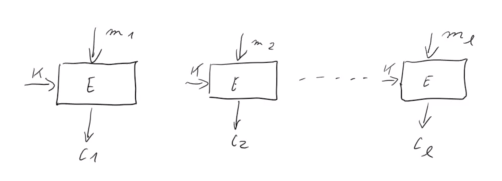
\includegraphics[width=1\textwidth]{images/ECB.png}
\end{center}

\noindent Questo sistema ha molte debolezze:
\begin{itemize}
    \item Blocchi che si ripetono producono lo stesso cyphertext, quindi sono riconoscibili;
    \item L'ordine dei blocchi, se scambiato, può generare messaggi ancora sensati. Noi possiamo ad esempio invertire i blocchi 2 e 7 e ottenere una manipolazione nota del plaintext pur non conoscendo il plaintext lavorando direttamente sul cyphertext (\textbf{malleabilità});
    \item È possibile fare un collage di blocchi provenienti da messaggi diversi ("Paga 100 euro a" -> "paga 10000 euro a").
\end{itemize}

\noindent L'unico vantaggio che ha è la possibilità di parallelizzare il lavoro. 

\section{Counter (CTR)}
CTR prevede di prendere di codificare un counter $ctr$ con il crittosistema $E$ e la chiave $k$, e mettere in XOR il risultato col blocco del messaggio da cifrare. Ad ogni cifratura, il counter viene incrementato di $1$. Il cyphertext finale è dato dalla ricomposizione dei risultati per ciascun blocco. 

\begin{center}
    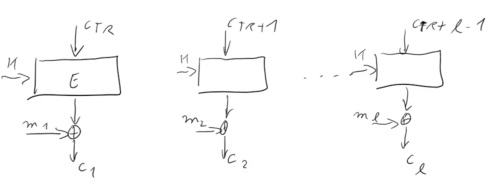
\includegraphics[width=1\textwidth]{images/CTR.png}
\end{center}

\noindent Con questo schema blocchi ripetuto generano cyphertext differenti e non è possibile fare collage di blocchi provenienti da messaggi differenti, a patto che il contatore sia differente. La debolezza di questo schema è il contatore: mittente e destinatario devono condividere il contatore e tenerlo sincronizzato. 

\section{Cypher Block Chaining (CBC)}
In CBC codifichiamo i blocchi del messaggio con il crittosistema $E$ e la chiave $k$ e, in ogni blocco successivo al primo, mettiamo in XOR il blocco con il cyphertext del blocco che lo precede. 

\begin{center}
    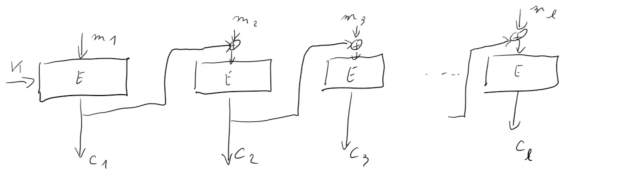
\includegraphics[width=1\textwidth]{images/CBC.png}
\end{center}

\noindent Il cyphertext del blocco precedente viene usato per modificare la sequenza di bit del blocco successivo. Con questo schema il collage non funziona e non esiste alcun contatore da mantenere condiviso. Il problema sta nel fatto che, se il cyphertext di un blocco contiene errori, questi vengono poi propagati in tutti i blocchi che lo seguono (es: in seguito ad errori di trasmissione).

Soffre inoltre del problema dei messaggi ripetuti. Questo problema può essere risolto aggiungendo un blocco casuale all'inizio del messaggio.

Vogliamo quindi trovare un sistema per evitare che l'errore di trasmissione si propaghi agli altri blocchi. Infatti qui, ad esempio, il blocco 

\section{Cypher Feedback}
Variazione del CBC che permette di trasmettere messaggi codificati bit per bit, piuttosto che blocco per blocco. Infatti in CBC il blocco $c_2$, ad esempio, non può essere inviato finché non abbiamo ottenuto completamente il blocco $m_2$.

\begin{center}
    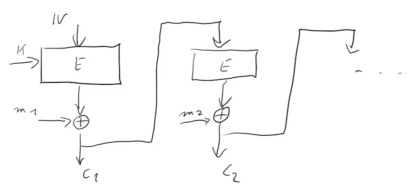
\includegraphics[width=0.7\textwidth]{images/CF.png}
\end{center}

\noindent Questo sistema utilizza un Initialization Vector $IV$ (da concordare con la controparte) che viene codificato con il crittosistema $E$ e la chiave $k$. Il risultato viene messo in XOR con il blocco da cifrare. Il risultato di questo viene usato sia come cyphertext del blocco corrente sia come nuovo $IV$ per la codifica del blocco successivo.

Il vantaggio di questo schema è che possiamo inviare il risultato dello XOR col blocco alla codifica del successivo bit a bit mentre viene generato. Lo schema che abbiamo costruito è a blocchi ma permette di fare la trasmissione a stream. Non è resistente ad errori di trasmissione. 

\section{Output Feedback}
In questo caso, diversamente da Cypher Feedback, inviamo alla codifica del blocco successivo l'output del crittosistema $E$, e non il risultato dello XOR.

\begin{center}
    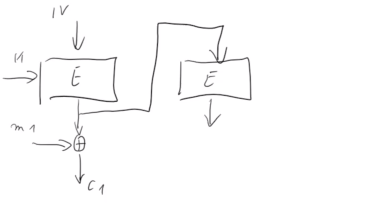
\includegraphics[width=0.7\textwidth]{images/OF.png}
\end{center}

\noindent Con questo scema un errore di trasmissione non ha influenza nel blocco successivo. Infatti, conoscendo l'$IV$, siamo in grado di calcolare tutte le uscite di ogni blocco senza dover leggere i cyphertext dei blocchi precedenti. Praticamente in ogni blocco usiamo una codifica della codifica di $IV$.